\documentclass[10pt]{article}
\usepackage[margin=0.78in]{geometry}
\usepackage{amsmath,amssymb}
\usepackage{graphicx}
\usepackage{booktabs}
\usepackage{microtype}
\usepackage{xcolor}
\usepackage{hyperref}
\usepackage{enumitem}
\usepackage{caption}
\usepackage{subcaption}
\usepackage{listings}
\usepackage{url}
\usepackage{fancyhdr}
\usepackage{multicol}

\hypersetup{colorlinks=true,linkcolor=blue!45!black,urlcolor=blue!55!black,citecolor=blue!45!black}
\setlength{\parindent}{0pt}
\setlength{\parskip}{4.5pt}
\captionsetup{font=small,labelfont=bf}
\pagestyle{fancy}
\fancyhf{}
\lhead{Full-Head Mapping Revisited}
\rhead{Kenneth Hurley}
\cfoot{\thepage}
\lstset{basicstyle=\ttfamily\small,breaklines=true,frame=single,backgroundcolor=\color{gray!5}}

\title{\textbf{Full-Head Mapping Revisited:}\\From Orthogonal Photo Projection and Multiresolution Splines\\to Landmark-Guided Multi-View Texture Synthesis}
\author{Kenneth Hurley\\Super-Genius\\\url{https://github.com/Super-Genius/full-head-mapping}}
\date{September 2026}

\begin{document}
\maketitle

\begin{abstract}
In the early 2000s, the \emph{Full Head Mapping} workflow addressed a practical content-creation problem: how to convert a small set of orthogonal photographs into a single texture covering an entire head. The original 3ds Max plug-in projected front and side photographs onto a pre-modeled head, selected source imagery according to surface-normal/view alignment, then used Burt--Adelson Gaussian/Laplacian pyramid blending to suppress seams before baking into a cylindrical destination map. This report reconstructs that method and generalizes it for Unity 6 as an arbitrary multi-view texture baker. The modern formulation rasterizes the destination UV atlas, projects each texel into calibrated source cameras, computes confidence from visibility, surface orientation, image borders, and user weights, and combines the projected images either by hard best-view selection, normalized weighted blending, or multiband blending. A confidence map and a source-provenance map explicitly distinguish observed from missing regions. We also describe a Blender alignment helper and optional integration points for facial landmarks, parametric head models, photogrammetry, and generative systems such as multi-image 3D models. The aim is not to replace observed identity texture with generated content, but to preserve photographed evidence first and use learned priors only where geometry or appearance is genuinely missing.
\end{abstract}

\textbf{Keywords:} multi-view texture mapping, head reconstruction, image mosaics, multiband blending, Unity, Blender, facial capture, texture synthesis

\section{Introduction}
A head is an awkward object to texture from photographs. A frontal image contains high-value identity information, but it provides poor observations of the ears and lateral skull. A profile image adds those regions while distorting or hiding the opposite side. Even when the geometry is already available, the practical problem is still one of registration, source selection, seam placement, exposure mismatch, and incomplete coverage.

The original \emph{Full Head Mapping} tool was developed for this production problem. The surviving Realistic3D description states that the goal was to map orthogonal photographs into one unfolded texture. The 3ds Max workflow assigned view directions to material IDs, planar-projected the source photographs, kept a cylindrical UV map as the final destination, and selected likely source views from the dot product between triangle normals and canonical view directions \cite{hurley_fullhead_web,hurley_shaderx_2002}. Hard selection left visible seams, so the tool adopted the multiresolution spline of Burt and Adelson \cite{burt_adelson_1983}. The original page reports roughly 20 seconds to generate the map on a Pentium III 500 MHz system.

That design still has useful ideas. What has changed is the surrounding tooling: cameras can be represented directly in Unity or Blender, facial landmarks can aid alignment, head priors such as FLAME provide fitted geometry, and generic multi-image 3D services can infer unseen shape. The modernization described here therefore preserves the historical deterministic texture pipeline while making geometry generation and AI completion optional stages.

\begin{figure}[t]
    \centering
    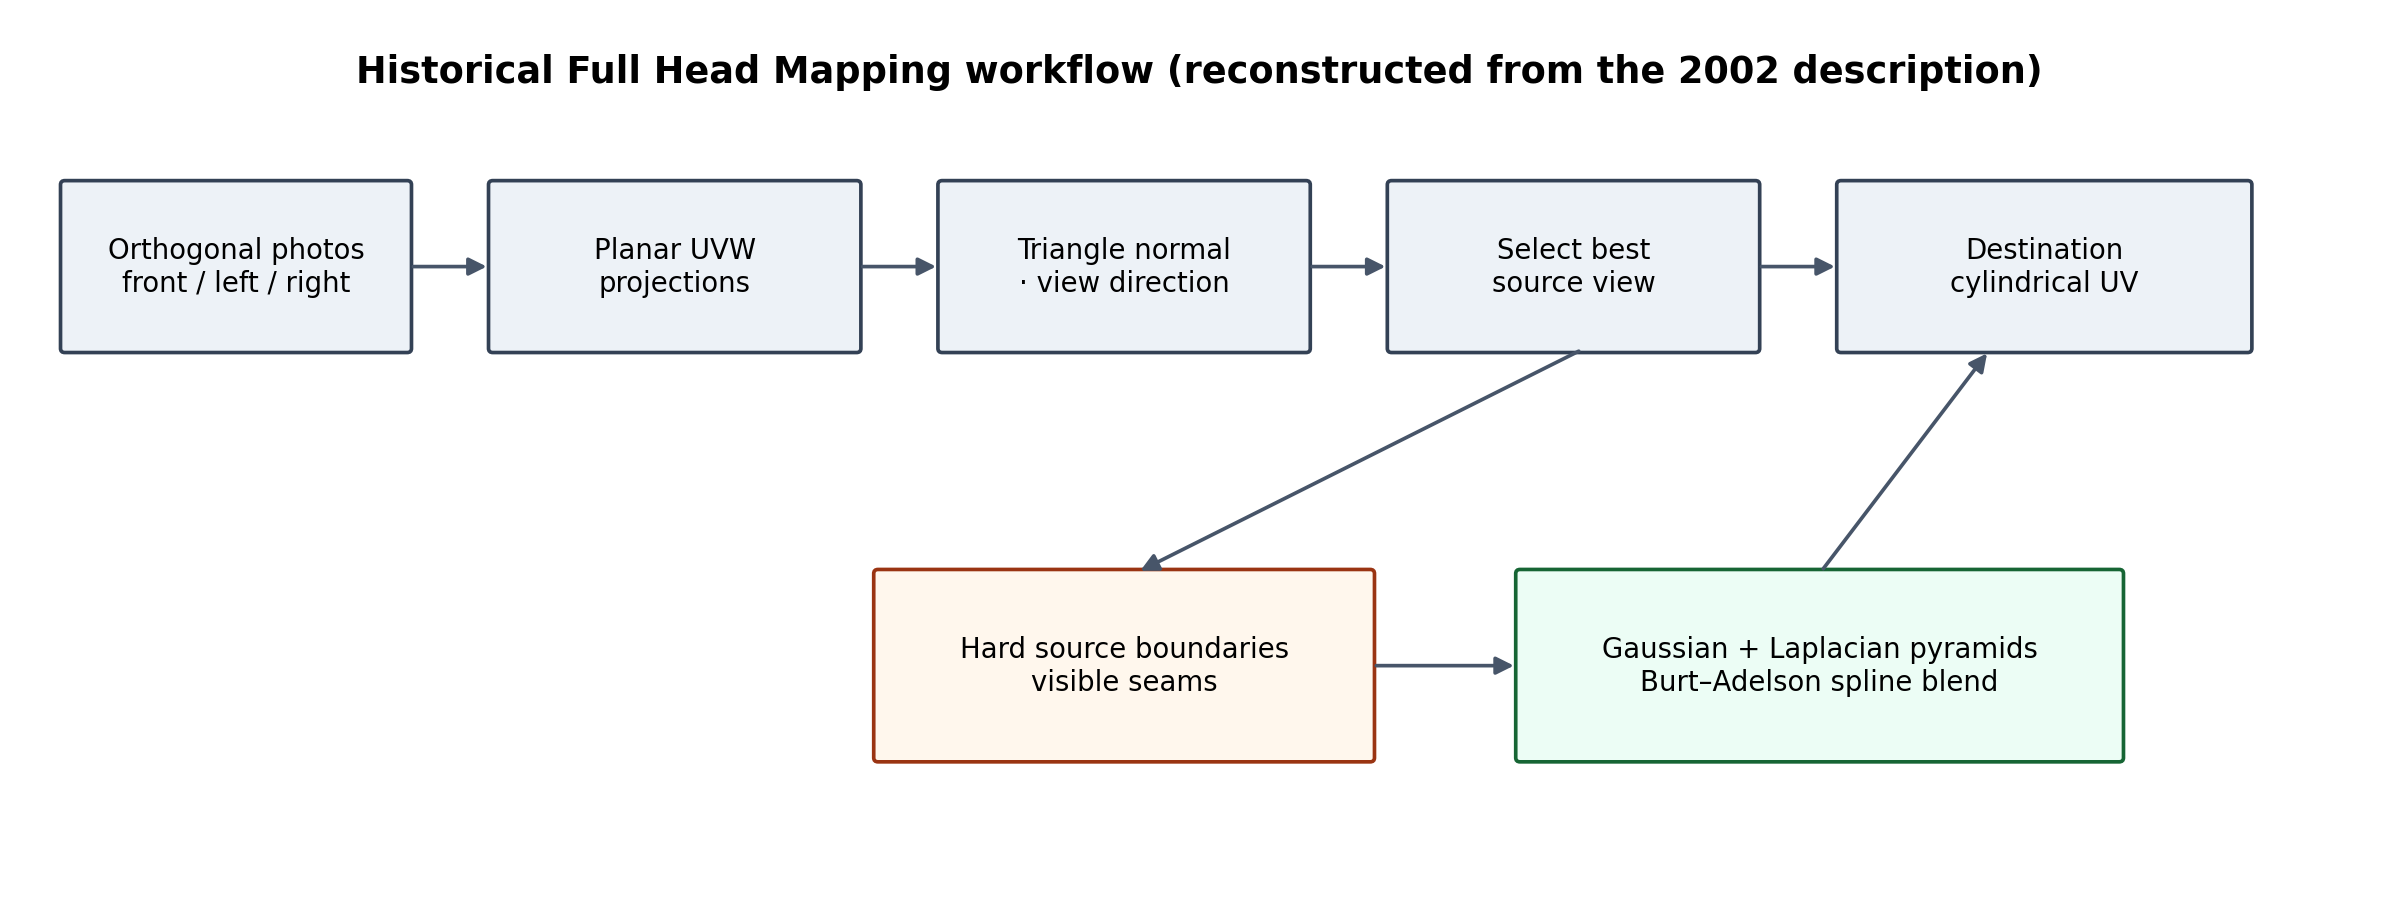
\includegraphics[width=0.98\linewidth]{figures/historical_pipeline.png}
    \caption{Reconstruction of the early-2000s Full Head Mapping workflow from the surviving article and ShaderX chapter. The central idea was not simply cylindrical mapping: source views were chosen by normal/view agreement and then joined with multiresolution spline blending.}
    \label{fig:historical}
\end{figure}

\section{Historical Method}
\subsection{Destination and source mappings}
The original head retained a destination cylindrical UV map. Separate photographs were planar-projected from the front and side directions. Material IDs encoded canonical source directions: right, left, top, bottom, front, and back, with a separate ID for the final cylindrical map \cite{hurley_fullhead_web}. This let the plug-in evaluate a source photograph on the surface and write the result into the final UV domain.

For triangle $t$ with representative unit normal $n_t$ and source direction $d_i$, the documented selection rule is naturally written as
\begin{equation}
    s_i(t)=\max(0,n_t\cdot d_i), \qquad i^*(t)=\arg\max_i s_i(t).
    \label{eq:historical_selection}
\end{equation}
The selected source gives a geometrically plausible view, but hard changes in $i^*$ create boundaries whenever neighboring regions choose different photographs.

\subsection{Multiresolution spline blending}
The original plug-in used the Burt--Adelson multiresolution spline rather than a single feathered blend. Their method decomposes images into spatial-frequency bands, blends low-frequency differences over broad regions, blends fine detail over narrow regions, and reconstructs the final image from the blended bands \cite{burt_adelson_1983}. This is particularly relevant for faces: exposure and broad shading differences should change slowly across a seam, while pores, eyebrows, hair, and other fine features should not be blurred over the same wide transition.

The historical page credits Peter Watje for the original program framework, Chris Hecker for texture-mapping code adapted into the tool, and Burt and Adelson for the pyramid blending method \cite{hurley_fullhead_web}. The original linked figure binaries are not reliably retrievable from the current site; Figure~\ref{fig:historical} is therefore an explicit schematic reconstruction rather than a claim to reproduce unavailable historical pixels.

\section{Modern Context}
The same problem can now be separated into three layers: camera/landmark registration, geometry, and texture synthesis.

\textbf{Camera and landmark registration.} Modern face-landmark systems can return dense facial landmarks and a facial transformation matrix. MediaPipe Face Landmarker, for example, exposes normalized landmarks and can optionally output facial transformation matrices and blendshape coefficients \cite{mediapipe_face_2026}. Such data can initialize or constrain the manual projector-camera alignment used in the first Unity implementation.

\textbf{Geometry priors.} FLAME models head shape, expression, jaw, neck, and eyeballs from thousands of aligned scans \cite{flame_2017}. DECA estimates detailed animatable facial geometry, albedo, expression, pose, and illumination from a single image \cite{deca_2021}. These methods are stronger geometry priors than a generic head mesh, but their software/model licenses must be handled separately from this MIT-licensed repository.

\textbf{General generative reconstruction.} Meshy currently accepts one to four images of the same object for multi-image 3D creation and also accepts multi-view images for texture guidance \cite{meshy_multiimage_2026}. That makes a generic generative model a useful baseline or optional geometry provider, but it is not equivalent to deterministic photo projection: it may infer appearance or geometry that was not directly observed.

\textbf{DCC projection.} Blender's UV Project modifier treats objects, including cameras, as projectors and supports up to ten projector objects; faces choose the closest/aligned projector, and camera projectors respect perspective or orthographic settings \cite{blender_uv_project_2026}. This closely echoes the old normal-based selection idea. The Blender helper included with this project focuses on camera/photo setup and interchange, while the Unity implementation performs the final multi-image bake.

\begin{figure}[t]
    \centering
    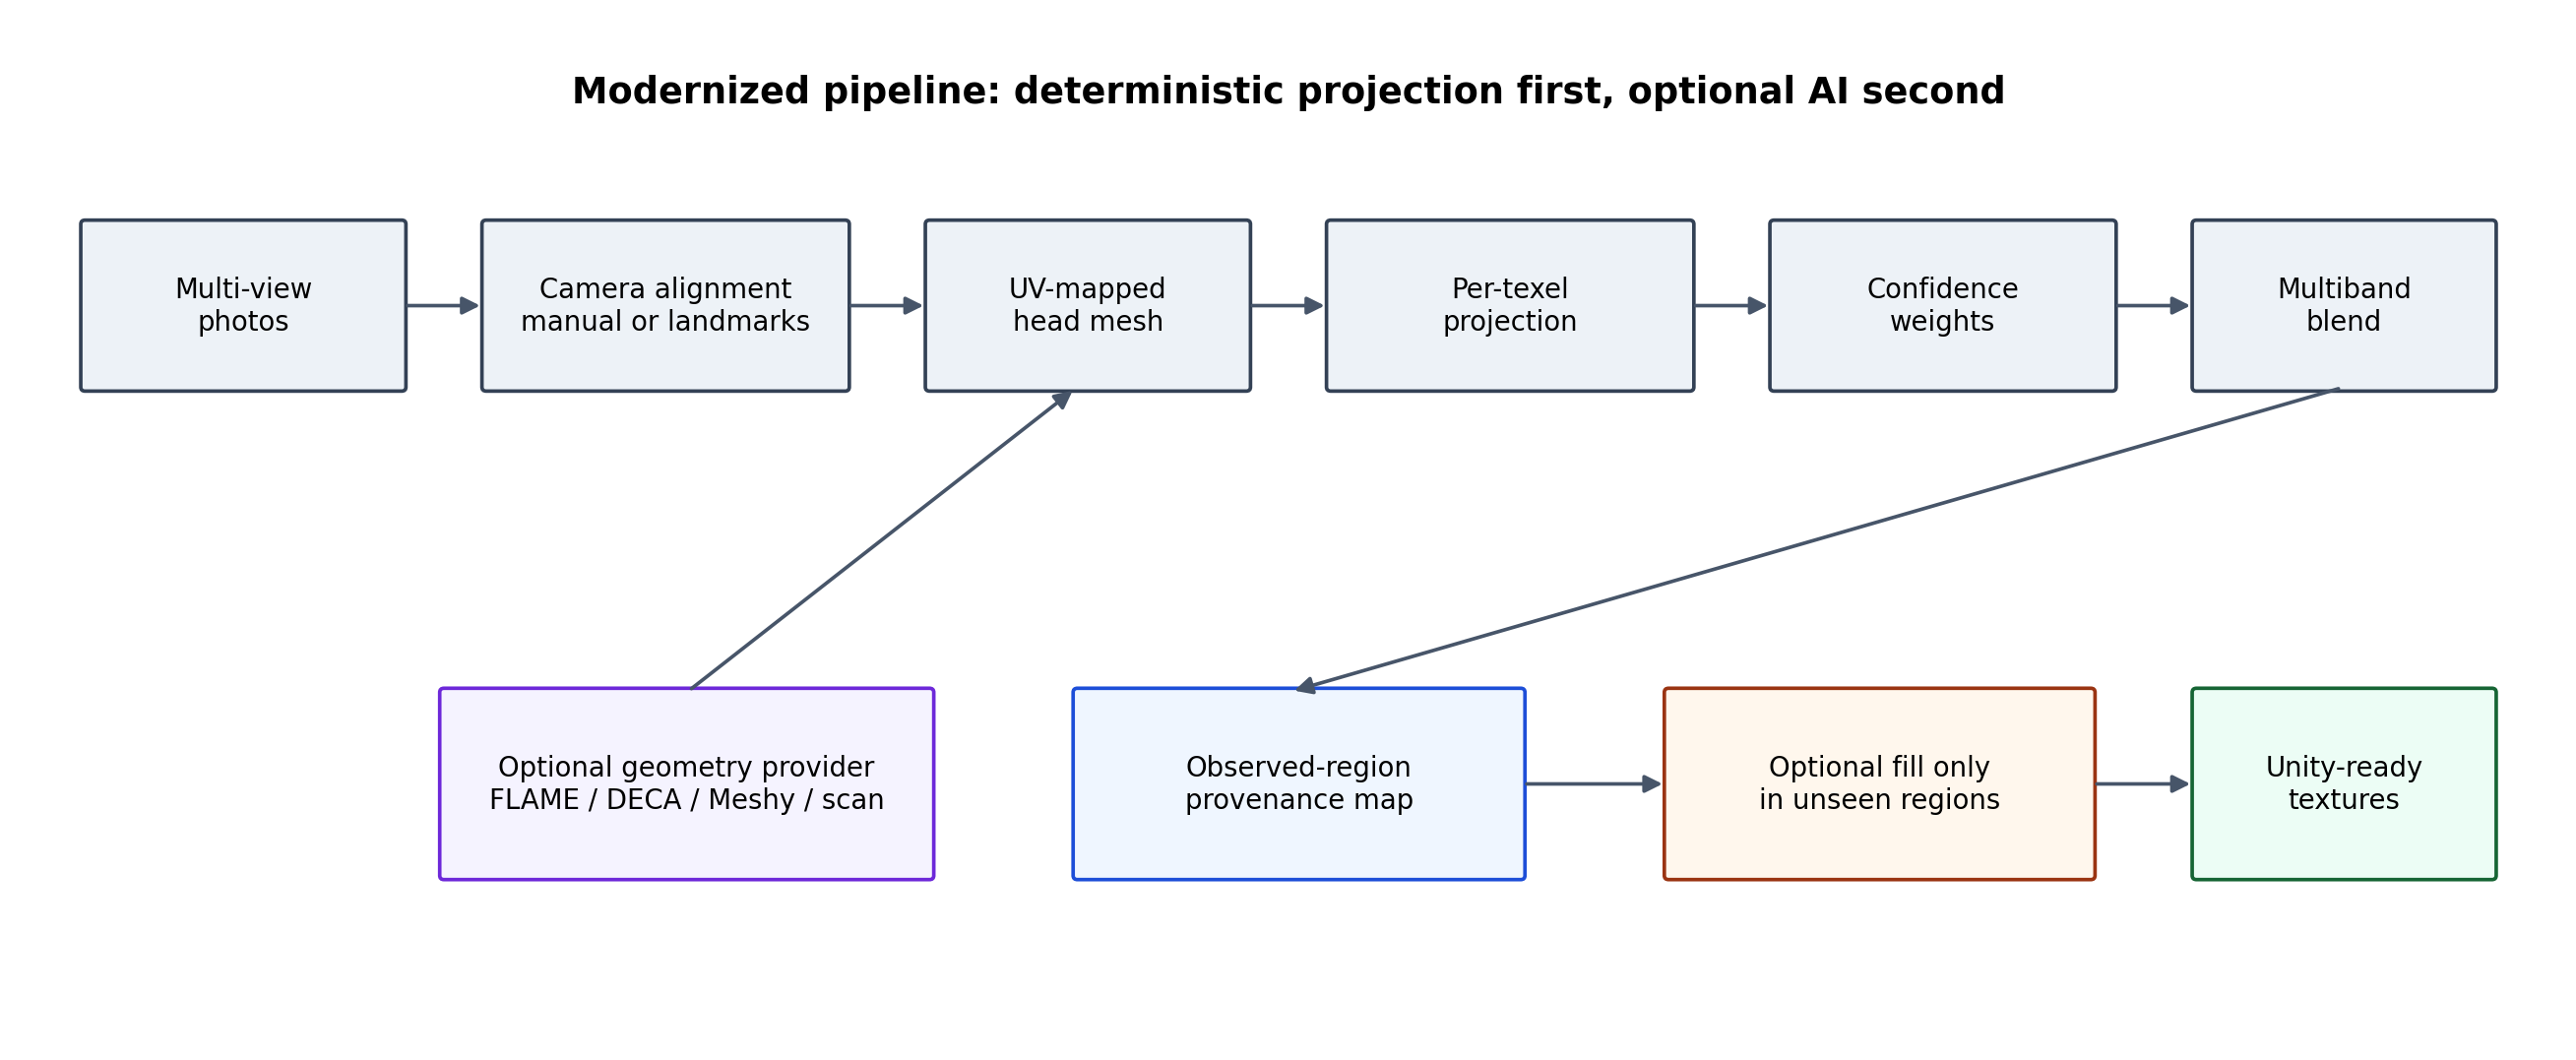
\includegraphics[width=\linewidth]{figures/modern_pipeline.png}
    \caption{Modernized architecture. Deterministic projection and provenance remain the core. Learned geometry or AI fill can be added before or after the bake without replacing photographed regions.}
    \label{fig:modern}
\end{figure}

\section{Generalized Multi-View Formulation}
Let $p$ be a texel in the destination UV atlas that maps to world-space surface point $x(p)$ with unit normal $n(p)$. Source $i$ has photograph $I_i$, camera projection $\pi_i$, camera position $c_i$, per-view scalar $\eta_i$, and a visibility indicator $V_i(p)\in\{0,1\}$. Define the surface-to-camera direction
\begin{equation}
    v_i(p)=\frac{c_i-x(p)}{\|c_i-x(p)\|}.
\end{equation}
The current implementation assigns confidence
\begin{equation}
    w_i(p)=\eta_i\,V_i(p)\,B_i(p)\,[\max(0,n(p)\cdot v_i(p))]^{\gamma},
    \label{eq:weight}
\end{equation}
where $B_i(p)$ softly suppresses samples near the source-image boundary and $\gamma$ controls how strongly oblique views are rejected.

\begin{figure}[t]
    \centering
    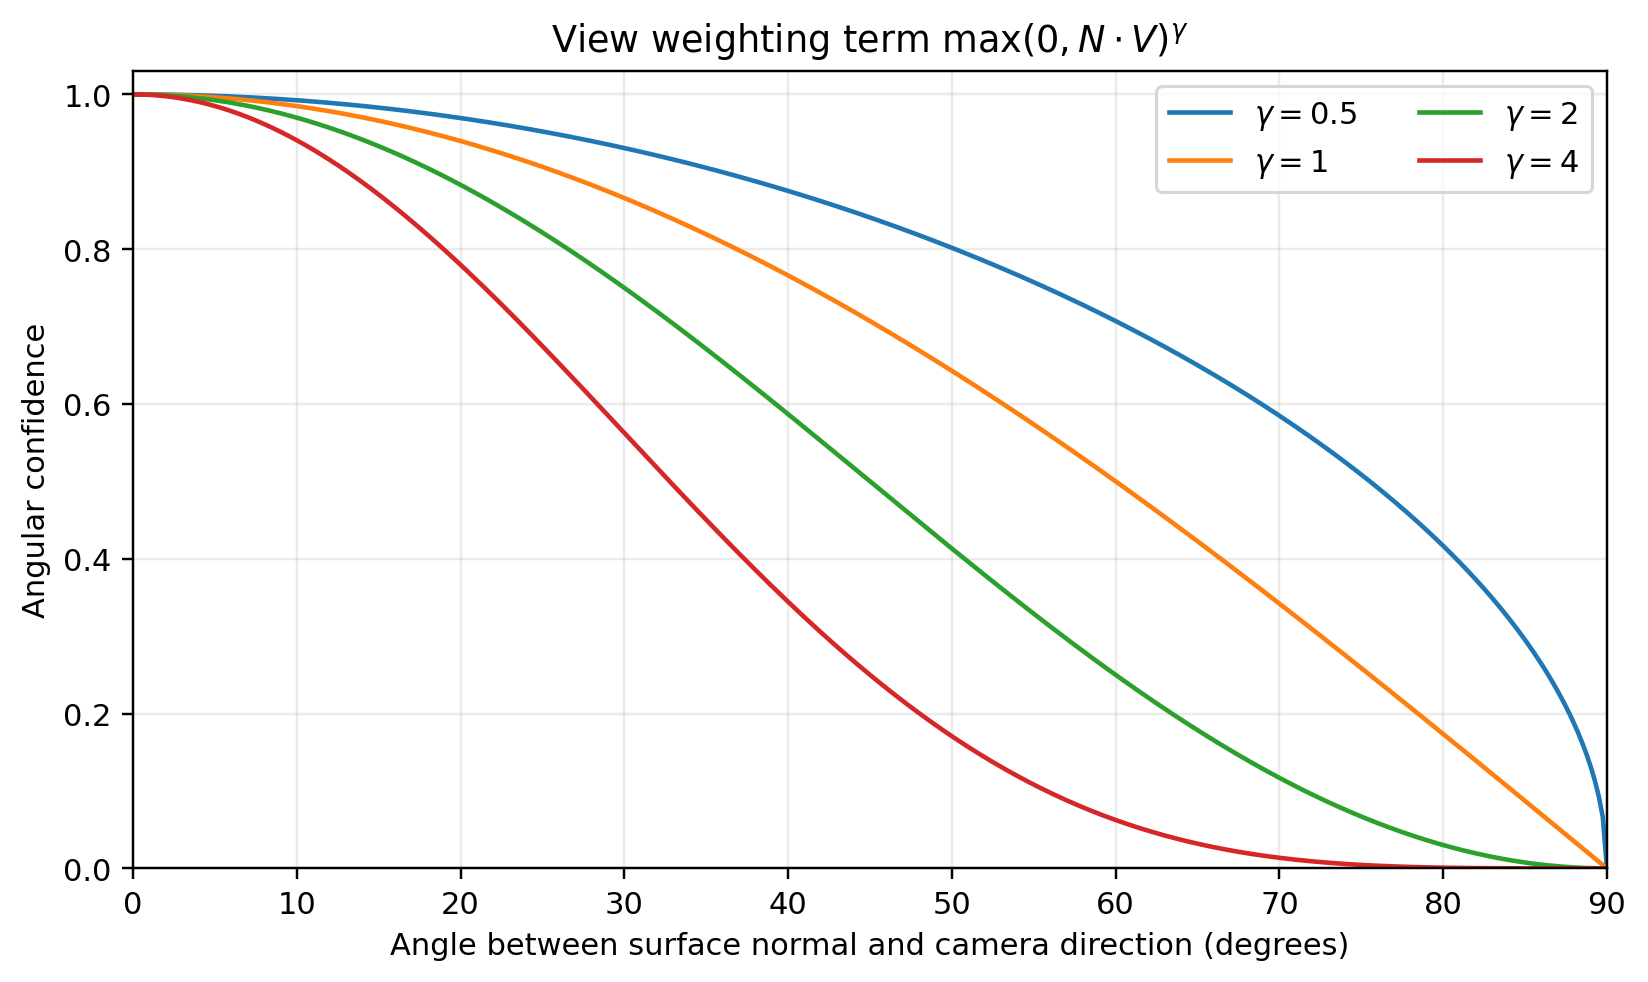
\includegraphics[width=0.72\linewidth]{figures/view_weighting.png}
    \caption{Angular confidence in Eq.~\ref{eq:weight}. Larger $\gamma$ prefers photographs that view a surface closer to head-on, reducing stretching but narrowing overlap between views.}
    \label{fig:weight}
\end{figure}

Three blend modes are useful for comparison:

\textbf{Best View} reproduces the spirit of Eq.~\ref{eq:historical_selection} at texel resolution:
\begin{equation}
    T_{best}(p)=I_{i^*}(\pi_{i^*}(x(p))), \quad i^*=\arg\max_i w_i(p).
\end{equation}

\textbf{Weighted} computes
\begin{equation}
    T_w(p)=\frac{\sum_i w_i(p) I_i(\pi_i(x(p)))}{\sum_i w_i(p)+\epsilon}.
    \label{eq:weighted}
\end{equation}
This removes hard source boundaries but can blur high-frequency detail where registration is imperfect.

\textbf{Multiband} constructs a Laplacian pyramid $L_\ell(I_i)$ for each projected source and a Gaussian pyramid $G_\ell(w_i)$ for each confidence mask. Each pyramid level is blended independently,
\begin{equation}
    B_\ell(p)=\frac{\sum_i G_\ell(w_i)(p)L_\ell(I_i)(p)}{\sum_i G_\ell(w_i)(p)+\epsilon},
\end{equation}
then the blended Laplacian pyramid is collapsed. This generalizes the historical spline from fixed orthogonal source IDs to any number of calibrated views.

\begin{figure*}[t]
    \centering
    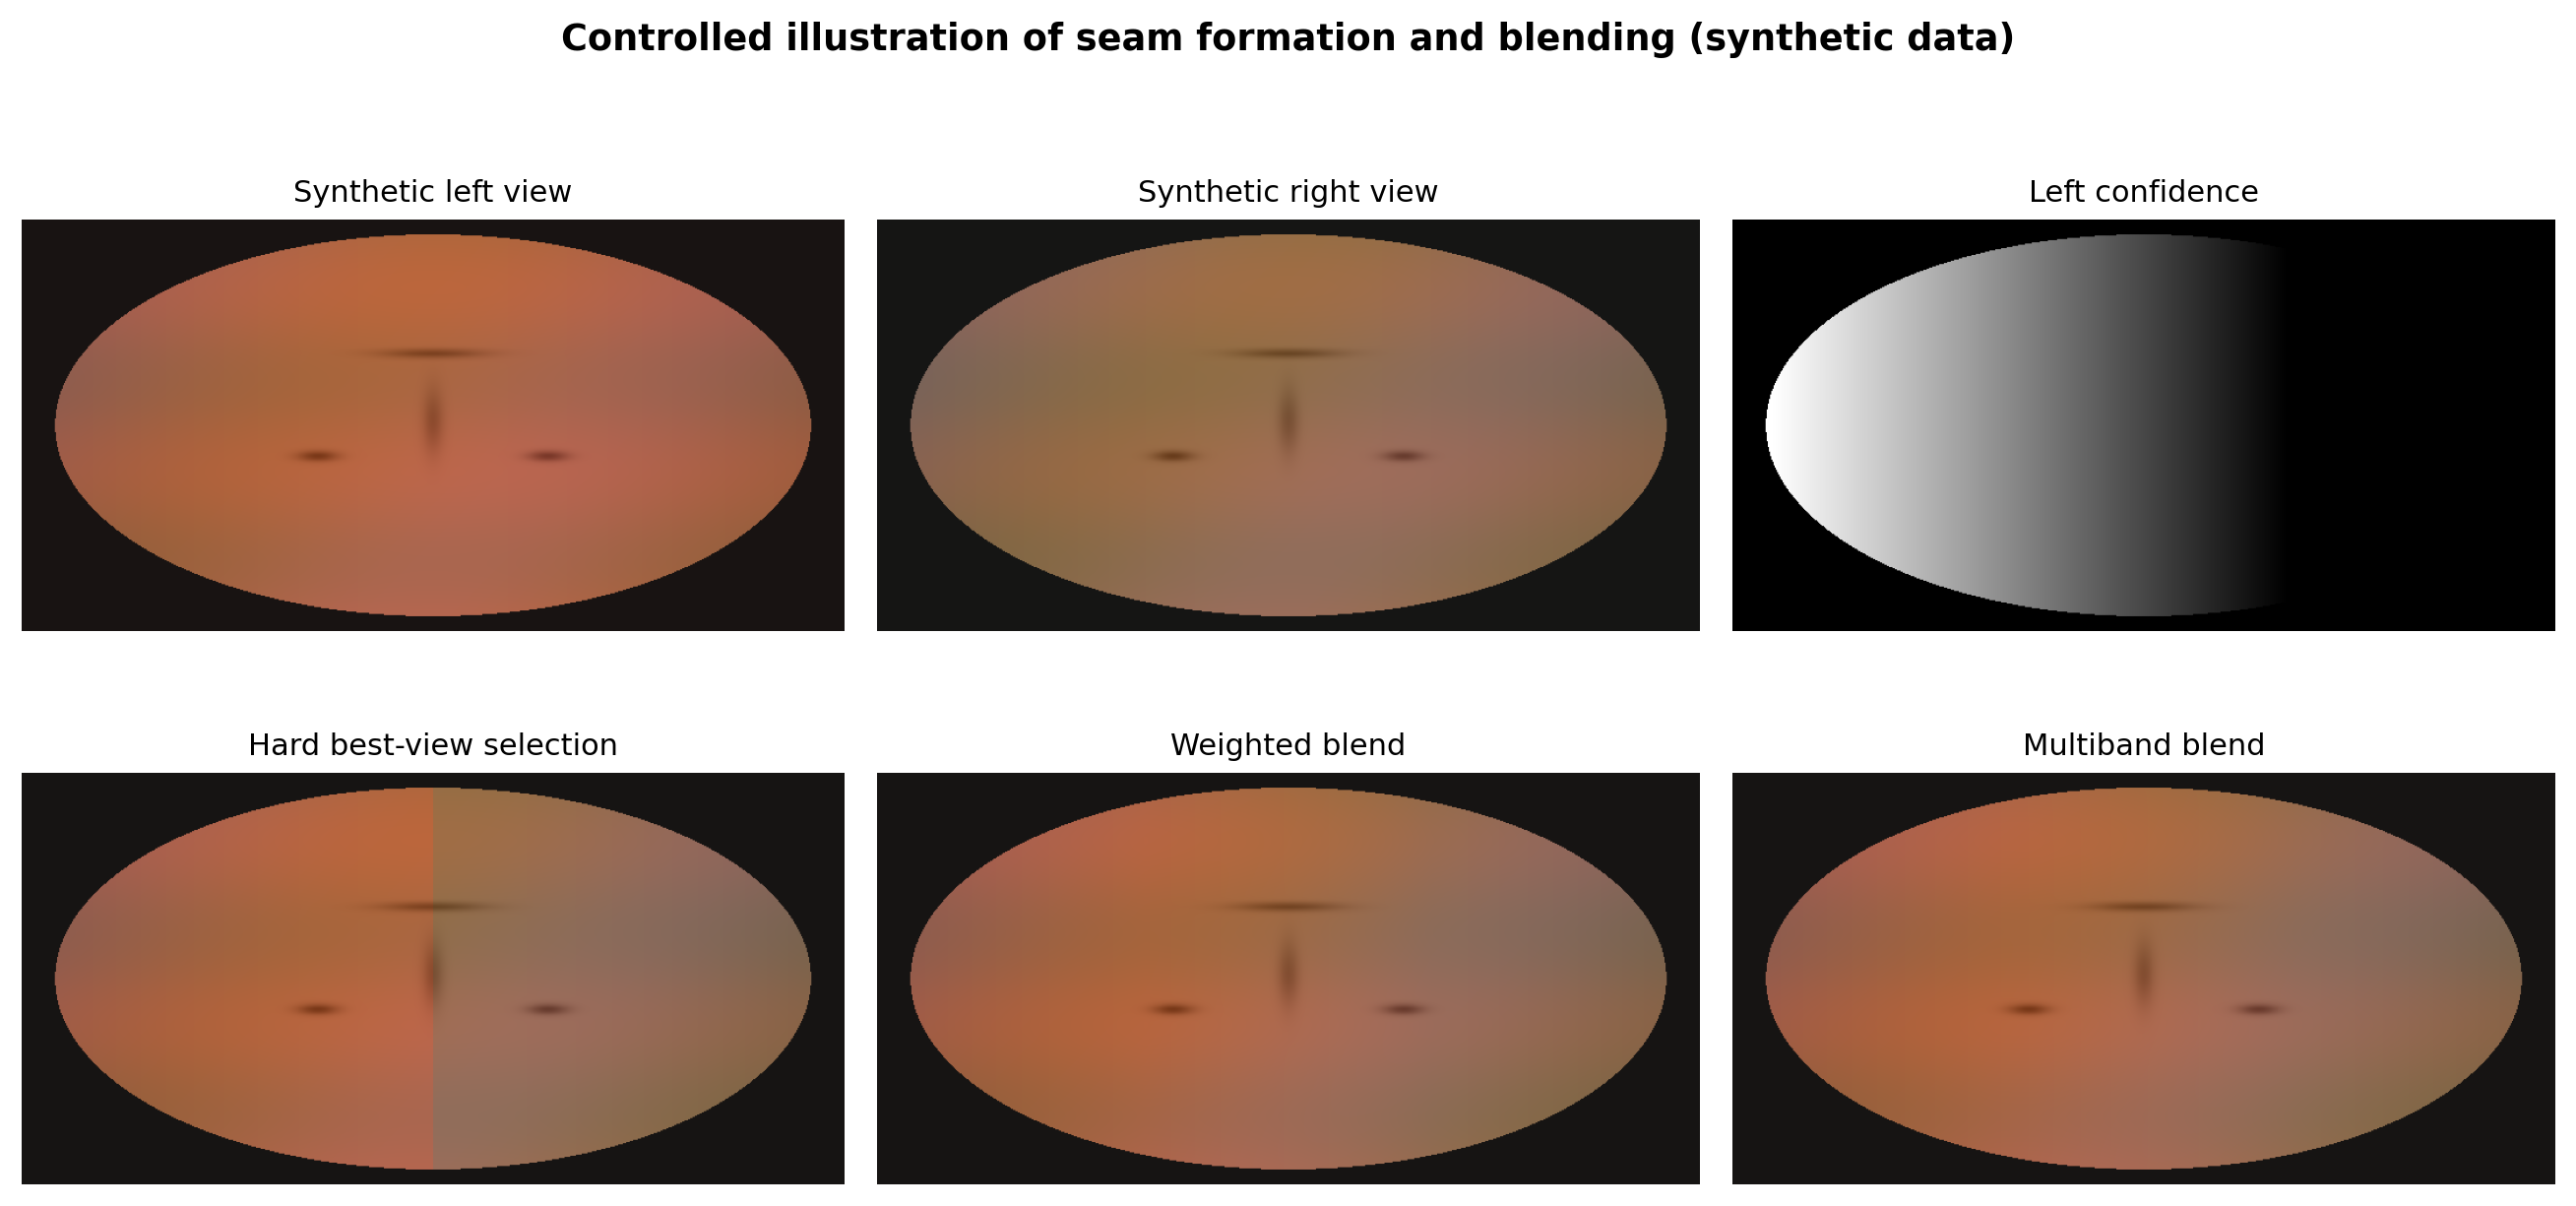
\includegraphics[width=0.98\textwidth]{figures/synthetic_blending_demo.png}
    \caption{Controlled synthetic illustration, not a photographed subject. Two source observations have deliberately different color balance and view confidence. Hard best-view selection creates a visible central discontinuity; weighted blending softens it; multiband blending distributes broad color changes while retaining more local detail.}
    \label{fig:blenddemo}
\end{figure*}

\section{Unity 6 Implementation}
The reference implementation is an Editor-only CPU baker so its behavior is easy to inspect and reproduce. The tool accepts an existing UV-mapped head and a list of photograph/camera pairs.

\subsection{UV-space rasterization}
For each triangle, its UV bounding box is rasterized in the destination atlas. Barycentric coordinates interpolate world position and normal for each covered texel. Each texel is then projected through each source camera. Sources are rejected if they are outside the camera, behind the camera, or back-facing. An optional physics ray test can reject occluded samples.

The baker stores a projected image and confidence mask for every source. Best-view and weighted results follow directly; multiband mode builds the Gaussian/Laplacian pyramids on these UV-space buffers. A simple overlap-based luminance gain can reduce gross exposure differences before blending. Missing regions can be dilated from neighbors as a conservative default.

\subsection{Confidence and provenance}
A key modernization is to keep uncertainty visible. We define a display confidence
\begin{equation}
    C(p)=1-\exp\left(-\sum_i w_i(p)\right).
\end{equation}
The baker writes this grayscale map alongside a provenance image whose hue identifies the dominant source. Figure~\ref{fig:provenance} shows the concept. Black denotes no direct observation.

\begin{figure}[t]
    \centering
    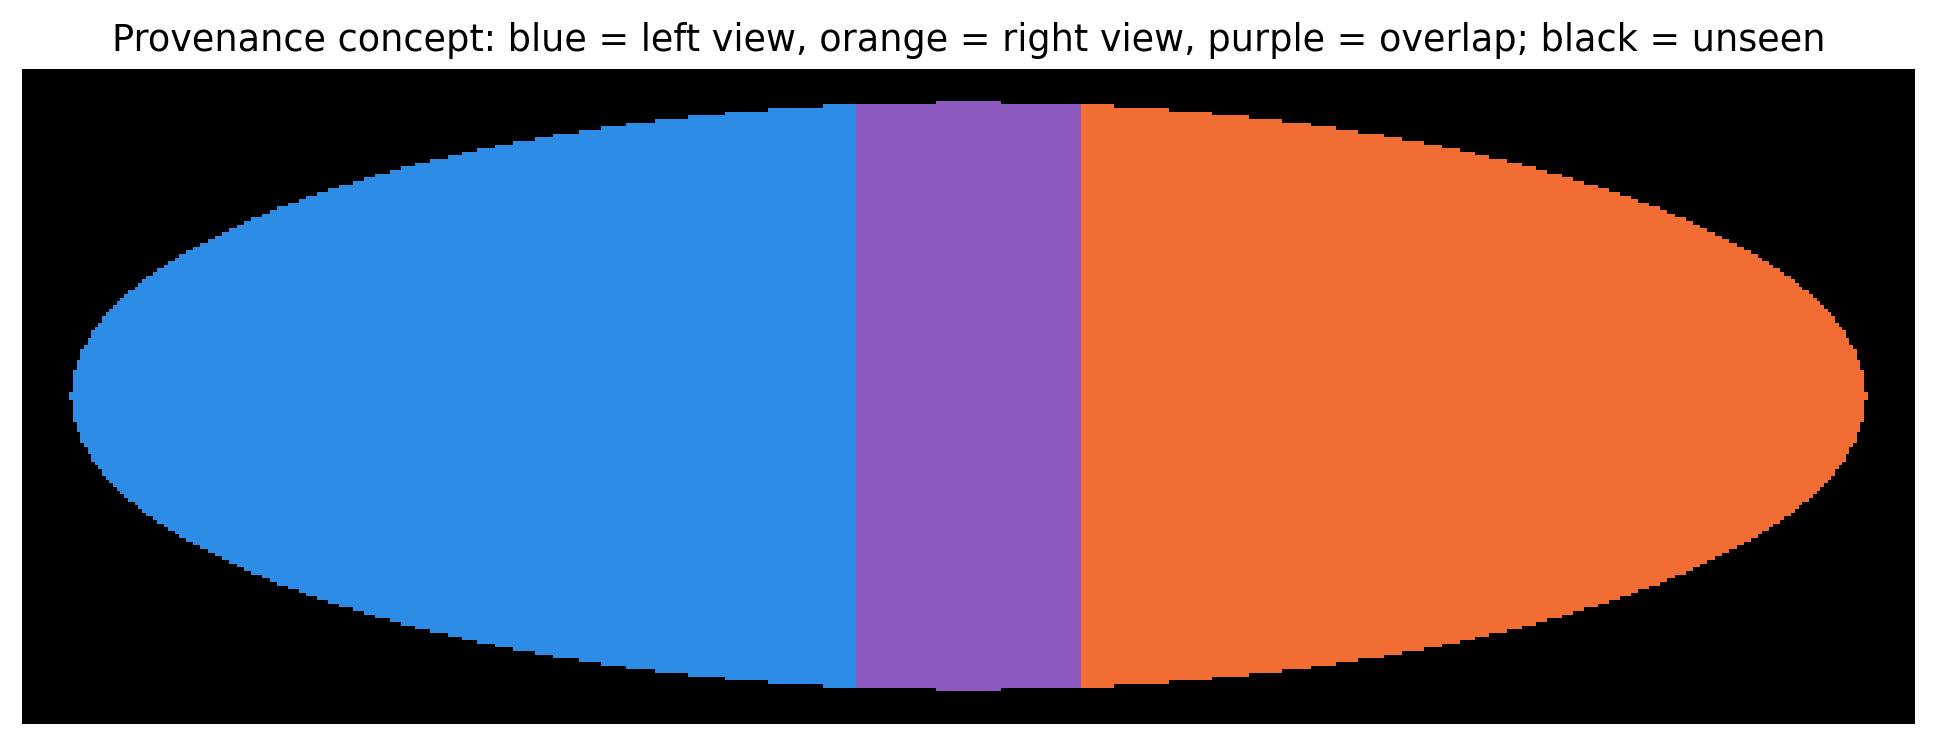
\includegraphics[width=0.82\linewidth]{figures/provenance_concept.png}
    \caption{Provenance-map concept. A production system can preserve this mask when later filling unseen ears, scalp, or rear-head regions so generated content is never confused with photographed evidence.}
    \label{fig:provenance}
\end{figure}

\subsection{Current workflow}
The package exposes \texttt{Tools > Super-Genius > Full Head Mapping > Open Baker}. The user can create standard front/left/right/back projector cameras, assign photographs, align cameras manually from the Scene view, select a blend mode, and bake albedo, confidence, and provenance textures. The implementation supports static meshes and baked snapshots of skinned meshes.

This first release deliberately uses CPU processing. Complexity grows with destination texels, triangle coverage, and source views. A compute-shader rasterizer and pyramid implementation are obvious next steps for interactive iteration at 4K--8K.

\section{Blender Workflow}
The repository also contains a small Blender add-on. It creates front/left/right/back projector cameras around a selected mesh, attaches images as camera backgrounds for registration, and exports a capture manifest. Blender is already capable of camera-based UV projection, making it a natural replacement for the old 3ds Max setup phase \cite{blender_uv_project_2026}. The add-on does not attempt to duplicate the full multiband baker; keeping the final blend in a shared core avoids two subtly different implementations.

A future version can move the projection/blending core into a standalone library or GPU compute path used by both applications. Until then, Blender is best treated as an optional camera/geometry alignment front end and Unity as the reference baker.

\section{Landmark-Guided and AI-Assisted Extensions}
The most useful role for modern learned systems is to reduce alignment effort and fill true gaps, not to overwrite good source photography.

\subsection{Landmark-guided camera solving}
Given corresponding 2D landmarks $q_{ij}$ in photograph $i$ and 3D landmarks $X_j$ on a template/fitted head, camera parameters can be refined by minimizing reprojection error
\begin{equation}
    E_i=\sum_j \rho\left(\|\pi_i(X_j)-q_{ij}\|^2\right),
\end{equation}
with robust loss $\rho$. MediaPipe landmarks can provide the 2D observations or an initialization \cite{mediapipe_face_2026}. The current repository defines the workflow but does not yet bundle a landmark model.

\subsection{Geometry providers}
The code exposes an \texttt{IHeadGeometryProvider} seam. A provider may return a deformed template, a FLAME/DECA fit, a photogrammetry result, a depth scan, or a generative reconstruction. FLAME offers a compact articulated head prior \cite{flame_2017}; DECA estimates detailed animatable geometry from a single image \cite{deca_2021}. Meshy's multi-image interface makes it a convenient generic comparison point for 1--4 views \cite{meshy_multiimage_2026}. None is made a required dependency.

\subsection{Observed-first completion}
For identity-sensitive capture, the provenance/confidence maps permit a stricter policy:
\begin{enumerate}[leftmargin=1.5em,itemsep=1pt]
    \item retain high-confidence photographed texels unchanged;
    \item multiband-blend overlaps between observed views;
    \item use conservative dilation for narrow holes;
    \item invoke generative texture or geometry completion only where $C(p)$ is below a threshold;
    \item preserve the completion mask alongside the final asset.
\end{enumerate}
This provides an audit trail absent from end-to-end generation.

\section{Evaluation Plan}
No quantitative result is claimed in this initial reconstruction. A useful evaluation should compare at least four pipelines on the same capture set: historical best-view selection, normalized weighted blending, multiband blending, and one external generated/fitted geometry baseline.

\begin{table}[h]
\centering
\small
\begin{tabular}{p{0.23\linewidth}p{0.67\linewidth}}
\toprule
\textbf{Measure} & \textbf{Purpose} \\
\midrule
Direct UV coverage & Fraction of destination texels supported by at least one photograph before dilation or generation. \\
Overlap disagreement & Color/gradient difference between valid source projections in shared regions; measures registration and exposure mismatch. \\
Seam energy & Image gradient change across dominant-source boundaries in the final atlas/render. \\
Landmark reprojection & Pixel error after manual or automatic camera alignment. \\
Geometry error & Distance to a reference scan when a controlled scan is available. \\
Artist time & Manual time required for camera alignment, masking, cleanup, and correction. \\
Perceptual identity & Human or appropriately governed face-similarity evaluation on held-out render views. \\
\bottomrule
\end{tabular}
\caption{Proposed evaluation measures. Identity evaluation should use consented data and preserve the distinction between research measurement and biometric deployment.}
\end{table}

The original workflow is historically interesting partly because it converted a manual art task into a deterministic bake on commodity hardware. The modern test should therefore report not only image error but also preparation and cleanup time.

\section{Limitations and Ethics}
The current Unity version assumes the target already has a usable, non-overlapping UV0 atlas. Camera calibration is manual. Visibility testing is optional and collider-dependent. Exposure normalization is scalar rather than spatially varying. Hair, translucent strands, eyes, teeth, and the mouth interior require their own capture/material strategies. Large pose or expression differences across photographs can create double features even with multiband blending.

A full-head capture is also biometric-like data. Photographs, fitted geometry, and identity textures should be processed only with the subject's consent and stored with suitable access controls. Generative completion can plausibly create visually convincing but incorrect identity details. The provenance map is included specifically to prevent inferred pixels from becoming indistinguishable from observed ones.

\section{Conclusion}
The early Full Head Mapping tool anticipated a structure that remains useful: choose photographs according to surface geometry, blend them at multiple spatial scales, and bake into one stable destination parameterization. Modern systems can improve every surrounding step---camera solving, geometry fitting, visibility, GPU acceleration, and hole completion---without discarding that core idea. The Unity 6 reconstruction therefore treats deterministic multi-view texture synthesis as the base layer and AI as an optional provider for geometry or genuinely unobserved regions. This keeps the workflow useful for research, games, and digital-human experiments while preserving a clear boundary between captured and inferred appearance.

\section*{Reproducibility}
Source code, Unity package, Blender helper, LaTeX source, figures, and the compiled paper are maintained at \url{https://github.com/Super-Genius/full-head-mapping}. The original historical description remains at \url{https://www.realistic3d.com/Full_Head_Mapping.htm}.

\begin{thebibliography}{9}
\bibitem{hurley_fullhead_web} Kenneth L. Hurley. \emph{Full Head Mapping}. Realistic3D.com, early 2000s. \url{https://www.realistic3d.com/Full_Head_Mapping.htm}.
\bibitem{hurley_shaderx_2002} Kenneth L. Hurley. ``Photorealistic Faces with Vertex and Pixel Shaders.'' In Wolfgang F. Engel, ed., \emph{Direct3D ShaderX: Vertex and Pixel Shader Tips and Tricks}, Wordware Publishing, 2002, pp. 296--318.
\bibitem{burt_adelson_1983} Peter J. Burt and Edward H. Adelson. ``A Multiresolution Spline with Application to Image Mosaics.'' \emph{ACM Transactions on Graphics}, 2(4):217--236, 1983. doi:10.1145/245.247.
\bibitem{flame_2017} Tianye Li, Timo Bolkart, Michael J. Black, Hao Li, and Javier Romero. ``Learning a Model of Facial Shape and Expression from 4D Scans.'' \emph{ACM Transactions on Graphics}, 36(6), Article 194, 2017. doi:10.1145/3130800.3130813.
\bibitem{deca_2021} Yao Feng, Haiwen Feng, Michael J. Black, and Timo Bolkart. ``Learning an Animatable Detailed 3D Face Model from In-The-Wild Images.'' \emph{ACM Transactions on Graphics}, 40(4), Article 88, 2021. doi:10.1145/3450626.3459936.
\bibitem{mediapipe_face_2026} Google. \emph{MediaPipe Face Landmarker}. Google AI for Developers, accessed September 2026. \url{https://ai.google.dev/edge/mediapipe/solutions/vision/face_landmarker}.
\bibitem{blender_uv_project_2026} Blender Foundation. \emph{UV Project Modifier}. Blender Manual, accessed September 2026. \url{https://docs.blender.org/manual/en/latest/modeling/modifiers/modify/uv_project.html}.
\bibitem{meshy_multiimage_2026} Meshy. \emph{Multi-Image to 3D API}. Meshy Documentation, accessed September 2026. \url{https://docs.meshy.ai/en/api/multi-image-to-3d}.
\end{thebibliography}

\end{document}
